%!TEX root = ../talk.tex

\chapter{Comparison of IoT Business Model}
\markboth{Comparison of IoT Business Model}{}
\chaptauthors{Matthias Diez, Christian Ott, Silas Weber}

\Kurzfassung{
	\begin{itemize}
		\item Explain why IoT and business models for it are relevant
		\item Present the method that is used to gain the results
		\item Summarize the results of the paper
	\end{itemize}
}

\newpage

\minitoc %Das Inhaltsverzeichnis

\newpage

\newcommand{\todo}[2][red]{\textcolor{#1}{#2}}
\renewcommand{\labelitemii}{$\diamond$}
\renewcommand{\labelitemiii}{$\circ$}

\section{Introduction and Problem Statement}
	The goal of this paper is fourfold, first a common ground is built, with the definitions and characterizations of IoT, business models and business model frameworks. Second, the basic business model framework concepts ``magic triangle'' and  Business Model Canvas are introduced. Third, the changes that were made to business model frameworks due to the development if IoT are highlighted, and lastly, the currently available IoT business model frameworks are presented and compared against each other.\\
	The rest of the paper is structured as follows. In Section~\ref{sec:iot} the term `Internet of Things' is introduced and its definition, growth, architecture and potential of IoT for business evaluated. Section~\ref{sec:bmf} presents the concept of business models and business model frameworks. Along with the definitions, two major `classic' business model frameworks are described. Section~\ref{sec:bmf_available} shows available business model frameworks that are adapted for IoT, Section~\ref{sec:bmf_comparison} will compare those frameworks and illustrate the results based on a model company. Finally, in Section~\ref{sec:eval} will evaluate the findings of the previous sections, the summery and conclusion will be presented in Section~\ref{sec:summary}. 
 
\section{Internet of Things}
\label{sec:iot}
	The term ``Internet of Things'' (IoT) has grown to one of the most discussed topics in academia and industry \cite{ju}. The phrasing was first used by Kevin Ashton during a presentation in 1999. From there IoT has become a new paradigm, it basically means the ``interconnection of physical objects, by equipping them with sensors, actuators and a means to connect to the Internet'' \cite{dijkman}.

	Even though the term ``Internet of Things'' is currently used by everyone, there is no common consent about its definition. The International Telecommunication Union (ITU) defined IoT 2012 in a recommendation as ``a global infrastructure for the information Society, enabling advanced services by interconnecting (physical and virtual) things based on, existing and evolving, inter-operable information and communication technologies'' \cite{itu}. Besides their view on IoT, other definitions were built, Atzori et al. identified three visions how IoT may be seen. As illustrated in Figure~\ref{fig:iot_visions} one is focused on the `things' getting connected over technologies like RFID, WLAN or NCF. The second visions is `Internet oriented', where anything connects with anyone . The third point of view is a `semantic oriented' vision, definitions in this direction can be found in literature. The the semantic oriented vision present thoughts on problems generated through the extremely increased number of connected `things', e.g. the challenging issues related to the representation, storage, interconnection, search and organization of information from IoT \cite{atzori}.\\
	Due to the differences in these visions, the definitions of IoT established by organizations or entities vary a lot depending on their specific interests, approach taken on the subject as well as their backgrounds. The convergence of these three visions illustrated in Figure~\ref{fig:iot_visions} can be seen as the overall paradigm of IoT, this is also the perspective this paper takes  on in the remaining sections. 
	
	\begin{figure}[ht]
	    \begin{center}
	    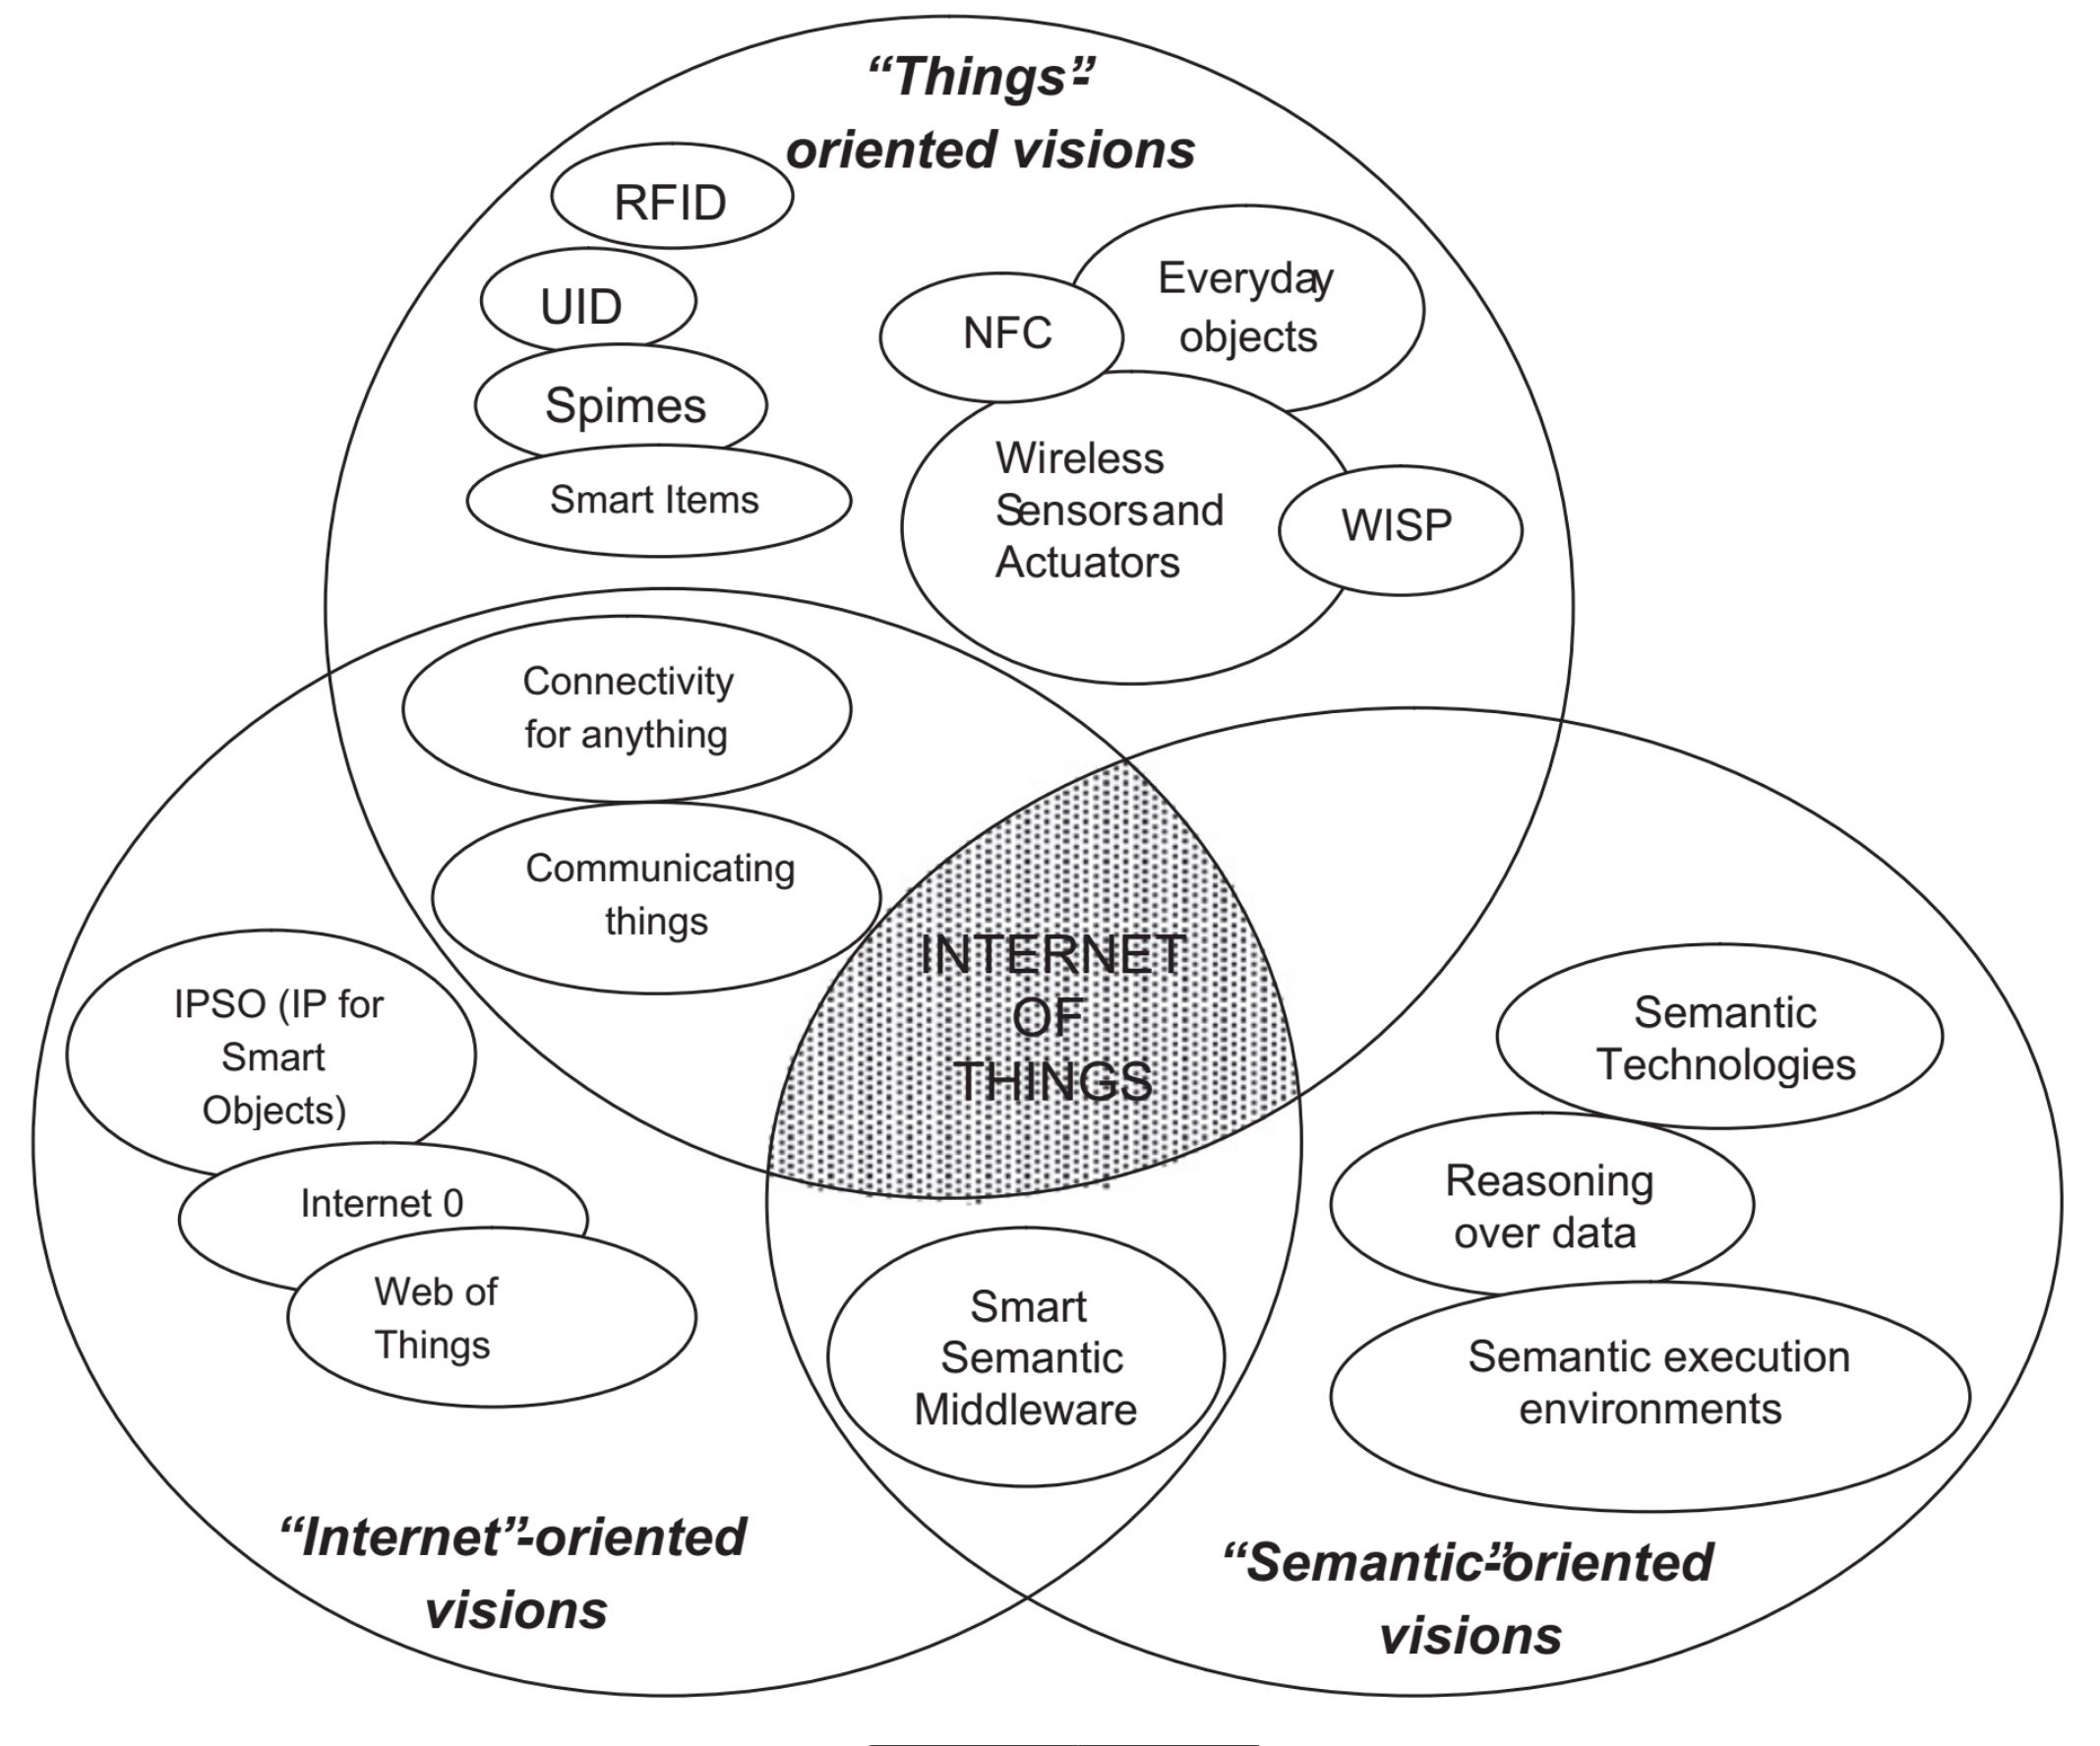
\includegraphics[scale=0.35]{Talk11/iot_visions.jpg}
	    \end{center}
	    \caption{``Internet of Things'' paradigm as a result of the convergence of different visions.}
	    \label{fig:iot_visions}
    \end{figure}

	The number of worldwide connected `things' is rapidly growing, in 2016 Gartner predicted up to 6.4 billion connected devices which will reach up to 20.8 billion by 2020 \cite{gartner}. Consequently organizations are more and more involved in IoT-related products, applications and services either in the development or as an investment \cite{ju}. Google acquired Nest for \$3.2 billion, a quickly growing smart thermostat company. Samsung bought SmartTings, an open smart home platform []. A lot of IoT companies emerge like LiFX as smart bulb company \todo{[] or TODO}. Telecommunication organizations invest in future technologies like 5G which was discussed in chapter \todo{??} of this seminar report. Governments increasingly acknowledge the importance of IoT, the United States supported a Smart Cities Initiative with \$160 million \todo{[]}, the Korean government planned \$5 billion investments in various IoT projects until 2020 \todo{[]}. The investments driven by national institutions as well as aggressive investments by companies in IoT would ``create new business opportunities and substantial social and economic benefits''\todo{[]}. 

	Even though there is no concrete definition what IoT is, there is some consent about the architecture of IoT. A Three layered application stack can be found in various research literature albeit the layers may be named differently they are semantically comparable \todo{[fleisch, ju, wortmann, ]}. A `thing' layer, which means a hardware-based sensing layer, it has the function to identify objects and collect information through sensors over short-rang and local networks \cite{ju}.\\
	The network layer transmits real-time data. It interconnects not only people to `things' but allows also an information flow between `things' autonomously. The data presented by the network layer can be used by companies to provide optimized and personalized services \cite{ju}\\
	The application layer is described by Ju et al. as a ``combination of data processing and intelligence analysis to meet the industry needs to realize an intellectualized industry''. The application layer allows companies to achieve ``different types of intelligent application solutions'' as well as the determination of business strategies\cite{ju}.

	The Internet of Things has a huge potential. On one side are the customers which enjoy new experiences through the new connected world, on the other side are the businesses getting involved in the IoT market, they hope \cite{ju}.\\
	
	\todo{TODO: potenzial beschriibe, f�r business und `private' bi business �berleitig zu BM und section BMF}

	\subsection{Cisco Internet of Things}
		This section takes a look at where business models stand today. Especially for business model frameworks that are built on an ecosystem view, standardization issues come into play. From Cisco's IoT Ecosystem study we look at the following three topics, namely players, market and standardization in regard to the current state of IoT.

		\begin{itemize}
			\item Players

		Cicso's study identified four types of players \cite{cisco}:

		\begin{enumerate}

			\item Commercial players in the off line world are mainly manufacturers producing smart appliances like smart phones, wearables or home automation devices but also smart automobiles etc.

			\item Commercial players in the online world are companies that provide IoT-enabling services. For example Amazon with Amazon Web Services, Google with Google Cloud Platform and Microsoft with Microsoft Azure which all offer platform and services that target the IoT market.

			\item Research and academia, according to Cisco will further incite the growth of IoT by creating new theories, products and materials. New innovations come from this player that stir up the market.

			\item Governments and utilities are the last big player identified by Cisco. They are the driving force for creating smart cities, the smart grid etc. They are the decision maker when it comes to regulation and policies for IoT technology and also play a key role in funding.

		\end{enumerate}
		
		\item Market

		There are numerous markets for IoT. Besides consumer goods like smart phones, smart homes and other smart appliances that most people already use or at least heard of, there are markets for:
		eHealth:  includes such things as virtual healthcare, bioelectronics sensors  like heart monitoring implant, real time monitoring of vital signs and fitness monitoring.
		Transportation:  ranges from smart public and private transport to other smart transportation systems such as services like Uber and Lyft or other car-pooling appliances. 
		Energy distribution: automation of the energy grid (smart grid) promises more efficiency and more resiliency on supply and demand side.
		Smart cities: is the idea that with the use of information and communications technology (ICT) network infrastructures are created to improve efficiency as well as development of all areas of urban life including social, business and cultural services.
		Manufacturing and distribution/ logistics: in the current trend of IoT in manufacturing, industry 4.0 or the so called fourth industrial revolution refers to the automation and data exchange based on cyberphysical systems and cloud computing creating a so called smart factory. 
		Public safety: early-warning system in smart cities can help preventing and mitigating catastrophes, but also road-traffic safety measures and emergency medical services etc. fall under this category.
		Agriculture: includes natural-resource management with GPS mapping technologies and sensors for analyzing crop yields, monitoring growth, measuring nutrient needs and many more.
		Big data analytics: with all those sensors and smart devices, a ton of data gets collected. This data properly analyzed can deliver great insights for their respective applications. This is why big data analytics will immensely benefit from IoT but also contribute as well.

		\item Standardization

		Cisco found that current IoT-specific standardization activities are restricted to specific vertical. This means standardization is only achieved for one specific scope of application for example healthcare, wearables, agriculture etc. This creates so called islands of disjointed and sometimes redundant development.
		Such a fragmentation is detrimental to the IoT market. Overcoming and preventing such fragmentations is the challenge. There are some major standard bodies active in IoT like the Institute of Electrical and Electronics Engineers (IEEE) or the World Wide Web Consortium (W3C). But not all of them have global reach.
		For businesses, application standards will enable interoperability between products.  This is needed for businesses that are part of an ecosystem and rely on interoperability. Furthermore, standardization improves flexibility, so that IoT businesses don't get stuck in specific industry because they are locked in. This flexibility furthers competition between companies which will in the end be beneficial for the end user and society.
	\end{itemize}

\section{Business Model Frameworks}
\label{sec:bmf}	
	\subsection{Definitions} 
		 A \textbf{Business Model} is ``a description of the value a company offers to one or several segments of customers and of the architecture of the firm and its network of partners for creating, marketing and delivering this value and relationship capital, to generate profitable and sustainable revenue streams'' [osterwalder 2005]. The concept of the business model became important in the 1990 as the Internet began to spread and became important since then [22]. There is no commonly accepted view what the business models should include [morris, osterwalder, schweizer]. Achtenhagen et al. stated that there has been a change from ``what business models are'' to ``what business models are for'' \cite{westerlund}. In various literature there seems to exist an agreement that a business model is `the way of doing business' for a particular firm \cite{westerlund}. The heart of each business model stands the goal of minimizing cost and maximizing revenue \cite{ju}.\\
		 Business models are composed of a variety of components. In business models commonly found components are customer segments, value proposition, channels, customer relationships, revenue streams, key resources, key activities, key partnership and cost structure[ osterwalder 2005]. These Components are the fundamental building blocks of the Business Model Canvas and, thus they are described in detail in Section~\ref{sec:bmc}. \\

		 A \textbf{Business Model Framework} is a tool to help a company in the development of its business model by presenting an overview over the business model components described above \cite{dijkman}.

	\subsection{Magic Triangle (Gassmann et al., 2013)}
		A successful business needs to offer products or services that there is a demand for and thus can be sold to make a profit. In short, a business has to create value. A company needs to have a strategy, a way of conducting business on an operational level that will result in long term financial success, else a business is not viable and will disappear from the market sooner or later.
		A business model can be seen as a logical abstraction describing how the business operates to make a profit. A business models hence is a core factor in deciding whether your business will be driven out of market or prosper. Having a suitable business model is essential. In fact, innovators of business have been found to be 6\% more profitable than product or process innovators (BCG 2008). With the spread of IOT new business models need to be developed to adapt to those technological changes in the environment and seize the opportunities that arise witch such a change. 

		But there seems to be a problem. Few managers can explain their company's business model ad-hoc, let alone define what a business model actually is \cite{gassmann}. They employ a simple conceptualization consisting of four central dimensions: Who, What, How, Value. 

		The Who, What, How and Value make up the Gassmann's \textbf{Magic Triangle}. The Who addresses the target customer Group. The What refers to the product or service to those customers. What is the value offered to the customer? The Value explains how the business model is financially viable. How is the value generated? It includes cost and revenue structures. The How addresses the process and activities as well as the resources and capabilities that are required for building and distributing the value propositions.		
					
		\begin{figure}[ht]
		    \begin{center}
		    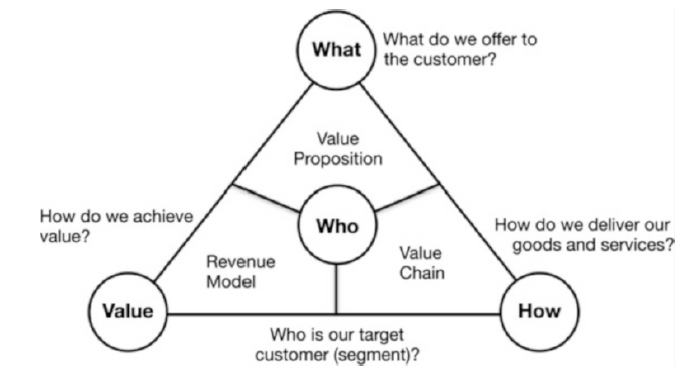
\includegraphics[scale=0.6]{Talk11/Figure1.png}
		    \end{center}
		    \caption{Gassmann's Magic Triangle}
		    \label{fig:m_triangle}
		\end{figure}
		The constellation of the magic triangle with the ``Who'' node in the middle is shown in figure \ref{fig:m_triangle}.
		Gassmann argues that reducing the business model to those four components allows for a simple, yet thorough enough view of the business model architecture.

		Creating new business models is not an easy task. It requires thinking outside the box, going beyond convention industry philosophy and can quickly become complex. People that are versed in change management will recognize some of the problem. First, why even come up with a new or improved business model? As long as there are still profits coming in, why take a risk and leave your comfort zone? Competition and environmental factor are always in movement. What works today may not work so well anymore in a few years. The syndrome known as the boiling frog syndrome states that gradually increasing problems are go unnoticed and or not dealt with until until it's too late to tackle them. A frog in pot with water won't jump out if the water is slowly brought to boil and when the water gets too hot for him, his muscles are too weak to jump out. Likewise, a business that has diminishing returns year after year may not be concerned about the the little loss between consecutive year. But when they realize the devastating loss suffered over multiple years there aren't any resources left to tackle the problem and they go bankrupt.

		Another problem is the not invented here syndrome, meaning that ideas not coming from within the company are disregarded solely because they come from the outside. As a consequence, business models should not just be copied from somewhere else but rather bring in external stimuli when generating ideas from within.

		Gassmann analyzed 250 business models in different industries from the last 25 years and as a result identified 55 pattern of business models that have served as the basis for new business models in the past. Then, together with selected companies they developed a construction methodology based on the fact that 90\% of all new business models have recombined previously existing ideas, concepts and  technologies. The BMI Navigator is the ready-to-use methodology for coming up with new business models consisting of the following three steps:
					
		Initiation: Describing the current business model is a good starting point. It creates a common ground for discussing the things that are done well and what needs improvement, and opportunities are open to be exploited. Also it get the participants started thinking in the ways of business models.

		Ideation: Open-minded team members are essential, preferably from different functions. This allows different viewpoint and thinking outside the box as well as overcoming the prevailing industry logic.
		
		Integration: Recombining existing ideas helps generating new business models. Gassmann condensed for this purpose the 55 business models into a set of pattern cards as shown in Figure~\ref{fig:pattern_card}. Each card has a title, a description and an example. The goal is applying different cards to the current model to see what would change in this situation. The cards should trigger discussions and act as a stimuli for new innovative ideas.

		\begin{figure}[ht]
			    \begin{center}
			    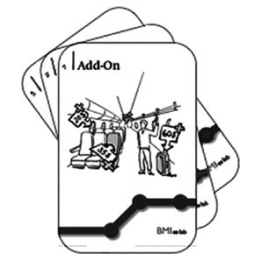
\includegraphics[scale=0.6]{Talk11/Figure2.png}
			    \end{center}
			    \caption{Pattern Card}
			    \label{fig:pattern_card}
			\end{figure}

		The last step is the integration. It's obvious that a newly generated idea cannot be implemented instantaneously. New ideas need to be gradually fleshed out into fully operational business models. Considering the new stakeholders, partners and consequences for the market is crucial.

	\subsection{Business Model Canvas (Osterwalder et al., 2010)} 
	\label{sec:bmc}
		The Business Model Canvas is a strategic management tool that was developed by Alexander Osterwalder in his doctoral thesis in 2004 and later published in book form by Osterwalder et al. \cite{osterwalder}. The tool supports business developers in gaining an overview about the key factors of their business. There are nine key factors explained by Osterwalder in detail and they are called `building blocks'. All of the building block can be aligned next to each other in a way that visualizes the mechanics of the business models (i.e. the interactions between the building block) and makes it easier to understand and discuss. The analog, pen and paper nature of the business model canvas allows it to be filled out in a team in order to stimulate creativity while finding a suitable business model for the business idea at hand.

		The usual order of filling out the business model canvas \cite{bmc} is by starting with the targeted ``Customer Segments'', then following with the \textbf{Value Proposition} to these customers and the `Channels' that allow us to deliver the described value to the customer. The value is not only delivered in a physical but there is an emotional `Customer Relationship' with the customer, too that needs to be considered. In exchange for the proposed value, customers are willing to pay money which make up the `Revenue Streams' of the business model. With this fifth building block, the money-generating revenue side of the business model canvas is complete.

		A business model always includes a cost side. In Osterwalder's canvas, the cost side consists of the following four building blocks: The `Key Resources' are human, financial, physical and intellectual resources that are critical to deliver the proposed value. But resources alone do not create value - they need to be used for `Key Activities' in order for the business model to be viable. As a business owner, the decision of what part of the value you create yourself and what you let other companies do for you is written down in the `Key Partners' building block. The costs induced by resources, activities and partners are finally collected in the `Cost Structure' building block.

		A `Customer Segment' can be a mass market, a nice market or a multi-sided platform. Business can have very diversified customer segments, with clear or unclear segmentation. It can be important to focus on the most important customers first.

		`Value Propositions' can have various characteristics such as the newness, performance, cost reduction potential or accessibility of the proposed value. The key questions to answer with this block is `What value do we deliver to the customer' and `Which customer needs are we satisfying?'. There can be multiple different value propositions per company.

		A company usually offers multiple `Channels' to serve their customers. Different customer segments may require different channels to get the product or service that the company offers. Also, the channel may differ along the different channel phases from Awareness, Evaluation, Purchase, Delivery to After sales.

		`Customer Relationships` differ strongly from company to company. Some forms of business models rely heavily on a personal customer relationship (e.g. barbershop) whereas for other companies the customers might not even be known because they help themselves in a self-service manner.

		`Revenue Streams` can stem from different sources and pricing models. A company can generate income through asset sale, fees for the usage, subscription, brokerage and licensing, or through advertising. Pricing models can be fixed (per feature, customer segment or volume) or dynamic (everyone gets a different price depending on the current context).
 
		`Key Activities' include all actions that are required to offer the `Value Propositions', to run the different `Channels` and maintain the `Customer Relationships' all of which generate the `Revenue Streams`.

		`Key Resources' include the physical, intellectual, human and financial assets of the company. The company pools these resources in order to turn them in an added value that can then be sold to customers.

		The decision to include `Key Partners' into a company's business model can have various reasons. It might be that the partner can provide a needed component of the model that is cheaper, that includes less risk and uncertainty for the company or that can not be provided by the company itself.

		The `Cost Structure' can be characterize along an axis from Cost driven (lowest costs in the market) to Value driven (best product/service in the market). Important characterizations of the cost structure include fixed and variable costs as well as the influence of economies of scale (the more you sell, the lower the cost per item) and economies of scope (the more diverse your offering, the more efficient a company can use its resources).	

\section{Available IoT Business Model Frameworks}
\label{sec:bmf_available}
	In this chapter, we will present and discuss different IoT Business Model Frameworks that are currently available in research papers.
	\subsection{IoT Business Model Patterns (Fleisch et. al, 2014)}
		Specific business model patterns can be found in the IoT environment were described in \cite{fleisch}. This is a good starting point to find out what areas an IoT business model framework has to cover. The analysis of 55 distinct business model patterns from Gassmann et al. \cite{gassmann55} yields two novel business model patterns that can be applied to an IoT business: `Digitally Charged Products' and `Sensor as a Service'.

		The pattern of a `Digitally Charged Products' is described as ``classic physical products are charged with a bundle
		of new sensor-based digital services and positioned with new value propositions'' in \cite[p. 10]{fleisch}. The components that cab be used and combined are ``Physical Freemium'' (free digital service with a paid product and offering paid premium services), ``Digital Add-on'' (digital services are sold to customer on an add-on basis to increase the value of the base product), ``Digital Lock-in'' (limit the digital compatibility), ``Product as Point of Sales'', ``Object Self Service'', ``Remote Usage and Condition Monitoring''. 

		\todo{TODO: explain in more detail?, explain layer model?, explain why it's not a framework as the others}

	\subsection{Adapted Business Model Canvas for IoT (Dijkman et al., 2015)}
		Dijkman et al. analyzed current research literature in order to create a business model framework for IoT applications. They searched for papers that contained the phrasing ``Internet of Things'' together with ``business model'', from the resulting 20 papers were 5 papers selected, only the ones that contained actual business models \cite{dijkman}. Two of the five papers were based on the business model canvas described in Section~\ref{sec:bmc}.\\
		Dijkman et al.  then identified the building blocks and building block types of business models through the selected papers and interviews with professionals working in the IoT business. Lastly he determined the relative importance of each building block or type through a survey.\\
		The result from Dijkman et al.'s research can be seen in Figure~\ref{fig:bm_dijkman}. The building blocks observed were equal to the building blocks from the Business Model Canvas described in Section~\ref{sec:bmc}. In order to `fill' the building blocks, the building block types presented by Osterwalder et al. in 2010 were, based on the interviews, merged, divided into multiple types, removed or extended by additional types \cite{osterwalder2010} \cite{dijkman}. The modified types can be seen in Figure ~\ref{fig:bm_dijkman} through the gray colored background.  

		\begin{figure}[ht]
			\begin{center}
		    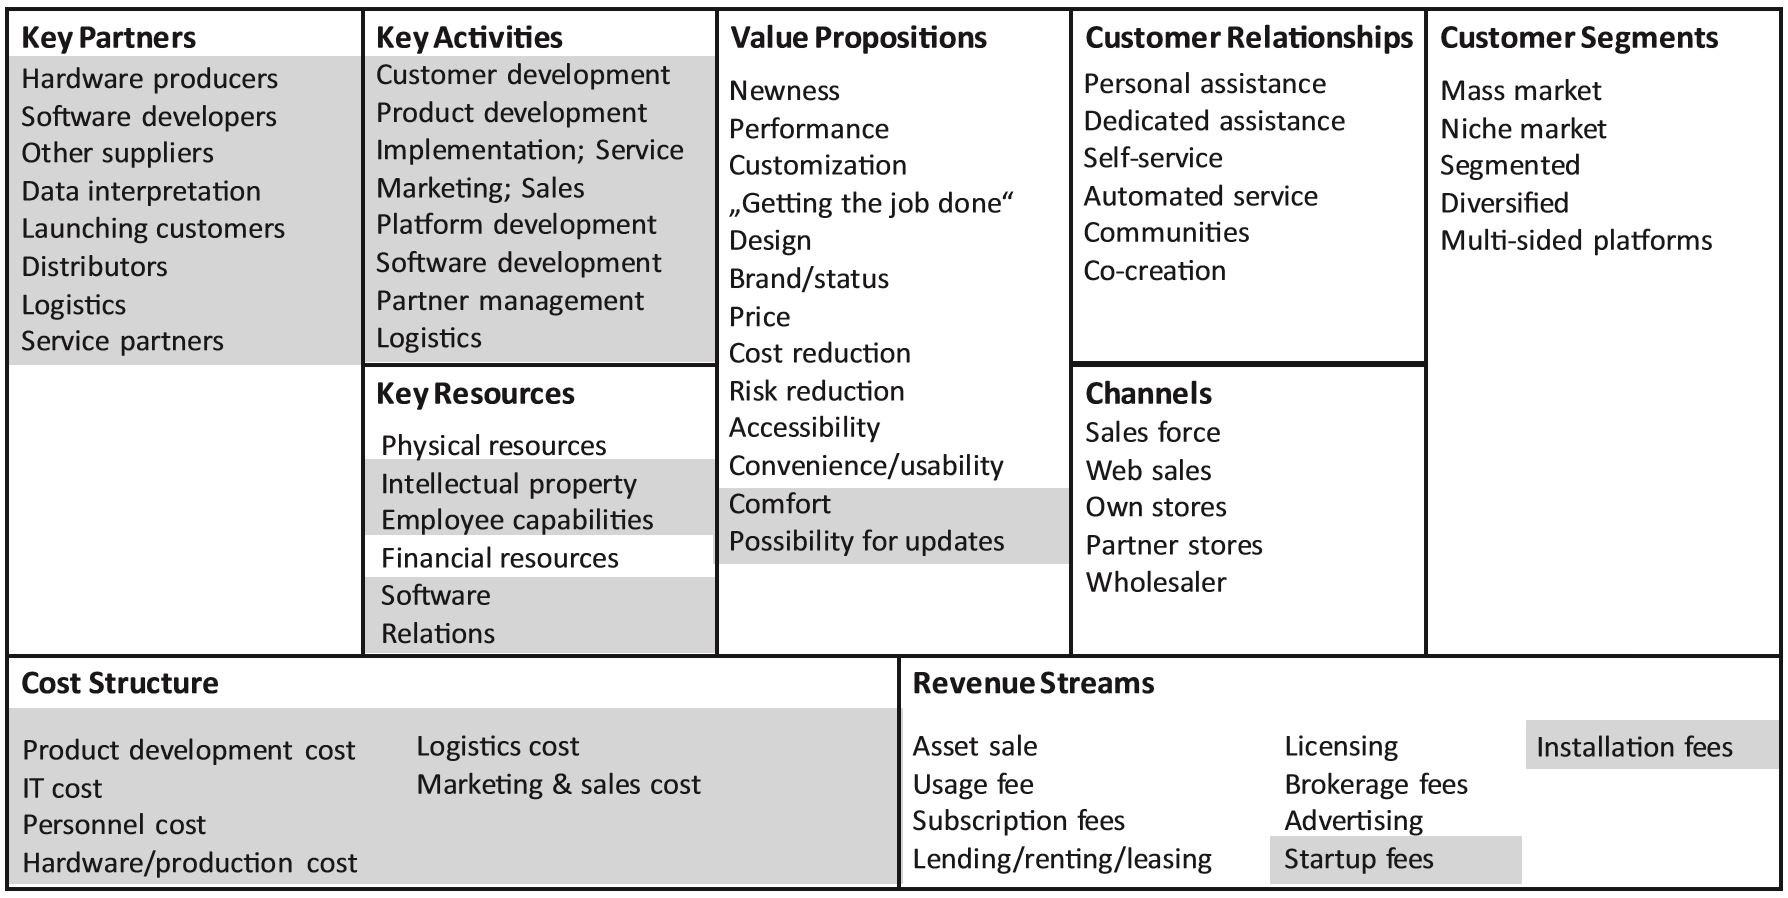
\includegraphics[scale=0.52]{Talk11/iot_canvas_dijkman.jpg}
		    \end{center}
		    %\caption{Business model framework for IoT applications with relative importance of specific types. \# < 0.05 significance, * < 0.02 significance, **  < 0.01 significance.}
		    \caption{Business model framework for IoT applications}
		    \label{fig:bm_dijkman}
		\end{figure}

		Based on the interviews and a survey, the relative importance of each building block was determined. Dijkman et al.'s work showed, that `value proposition' is most important in IoT business models. Furthermore, `customer relationship' and `key  partnerships' were also considered as more important by the interviewees, all other blocks had comparable importance results with  `channels' being a bit less important.\\    
		
		\todo{TODO: wrapup}
		\todo{TODO: explain most significant building block types in detail}

	\subsection{Ecosystem Business Model Value Pillars (Westerlund et al., 2014)}
		Westerlund et al. moves from seeing IoT mainly as a technology platform to viewing it as a business ecosystem. Thus there is a shift from the traditional business model of a firm to designing ecosystem business models. Such an ecosystem business model is composed of value pillars, creating and capturing value. They identified three major challenges for designing ecosystem business models namely diversity of objects, immaturity of innovation and unstructured ecosystems.

		As businesses from centralized toward decentralized and distributed network structures, they become part of a complex business ecosystems. A business ecosystem can be seen an organization of economic actors. Those actors' business activities are anchored around a platform. It's is argued that such systems are more than the sum of its part and hence ``operations of the system cannot be understood by studying its parts detached from the entity'' \cite{westerlund}.

		Existing business model frameworks such as the magic triangle and the business model canvas described above are arguably not adequate enough when it comes to analyzing such ecosystems. With IoT the interdependency of actors in an ecosystem gains importance due to the networks inherent to such ecosystems.

		As for all business, making money is essential. Three problems were identified  when it comes to making money in the Internet of Things.

		Diversity of object refers to the variety of different types of connected objects. Without a widespread standardization, it will be difficult to be efficient in an ecosystem. Managers will face a difficulty when trying to bring the objects, businesses and consumers together. Things can integrate with other things, requiring specific business logics.

		Immaturity of innovation refers to the current multitude of emerging technologies and components as well as innovations that have not yet matured into products and services. For IoT to be successful, modularized objects with of a `plug and play' type are needed.

		With unstructured ecosystems, the problem of lacking governance and underlying structures is addressed. Unstructured ecosystems may lack essential participants for example IoT operator or potential customers. New business opportunities arise when new relationships in new industries are built and already existing connections are extended,

		The ecosystem business model framework helps managers designing feasible business models that overcome these previously discussed problems and fit in the ecosystem nature of IoT. 

		The proposed framework consists of four key pillars, value drivers, value nodes and value exchanges shown in figure \ref{Westerlund pillars}:

			\begin{figure}[ht]
			    \begin{center}
			    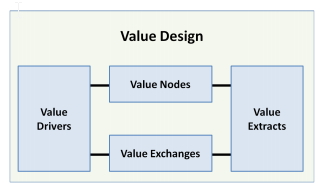
\includegraphics[scale=1.0]{Talk11/westerlundpillars.png}
			    \end{center}
			    \caption{The four pillars}
			    \label{Westerlund pillars}
			\end{figure}

		There are different \textbf{value drivers} in an ecosystem. Those value drivers are composed of both individual and shared motivation of the participants in the ecosystems. The shared motivations i.e. the shared value drivers are crucial for creating a win-win trustworthy ecosystem. Without a long term relationship between the actors with mutual respect of their business goals, the ecosystem will fail. Each value driver also serves as an individual value node's motivational factor. Examples of shared value drivers may be cybersecurity and improved customer experience.

		\textbf{Value nodes} consist of various actor, activities and processes linked with other nodes to create value. Further, these nodes also have autonomous actors. Here come the smart things into play. These autonomous actors may be sensors, smart machines or other intelligence. Value nodes are heterogeneous. They could be organizations, networks of organizations or even network of networks.

		\textbf{Value Exchanges} are the exchange of value between but also within different value nodes in the system. The value can be resources, knowledge and information thus they are tangible as well an intangible. Value exchanges are best described as a flow that powers ``the engine''. Value exchanges are important because they describe how revenues are generated and distributed in the ecosystem.

		As not all created value is meaningful in regard to commercialization, only specific parts of created value make sense to extract. \textbf{Value extract} refers to the part of the ecosystem that extracts value. That means it focuses on what can be monetized and what the respective nodes and exchanges are for the value creating and capture. The concept of value extract is useful to have a restricted view on what is actually relevant in the ecosystem to monetize on. Each business in the ecosystem needs to have something that is beneficial for them from the business point of view. Value extract can be single activities, automated processes, individuals, commercial organizations, non-profits or even groups of organizations or networks with their respective value flows between their nodes.

		Westerlund's et al. business model framework is heavily focuses on the value part of business models. Under the concept of value design those four value pillar described above come together in a single picture. Value design is an architecture mapping the foundational structure of the ecosystem business model. It provides boundaries for an ecosystem and gives a pattern of operation.

	\subsection{Three-dimensional collaborator Model (Chan, 2015)}

		The three dimensional collaborator model presented by Chan \cite{chan} builds on on a model described by Holler et al. \cite{holler}. The three dimensions of Chan's model are Who, Where and Why. On first sight, those dimensions seems similar to the nodes in Gassmann's et al. magic triangle proposition but the differences become evident once the meaning behind the three dimensions is investigated. The `Who' describes the collaborating partners that build the value network. The `Where' refers to sources of value co-creation and lastly the `Why' describes how partners actually benefit from collaborating withing the value network \cite{chan}. Figure \ref{Chan framework} shows the table of the proposed framework.

		\begin{figure}[ht]
		    \begin{center}
		    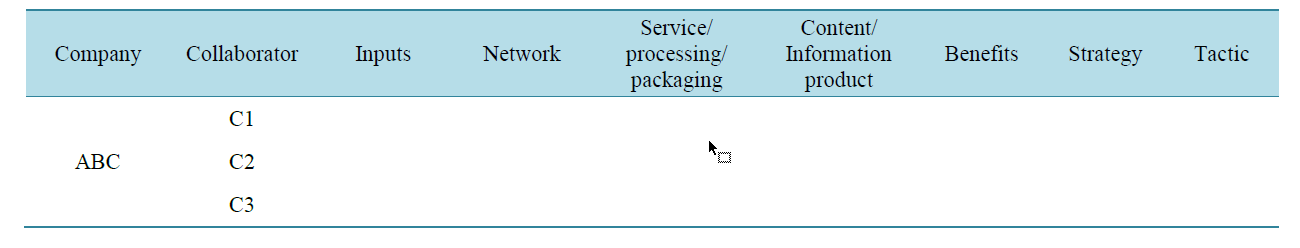
\includegraphics[scale=0.5]{Talk11/chan.png}
		    \end{center}
		    \caption{Chan's business model framework}
		    \label{Chan framework}
		\end{figure}

		Chan applied his framework on multiple case studies to explore the why, what and how elements of the business model. A look at one example of the Hong Kong Communications Co., Ltd (HKC) company helps to understand how the framework can be filled out for a use case. The Wong Tai Sin Temple in Hong Kong is a popular tourist attraction. With over 5 million visitors per year, the information board at the temple containing detailed information about the temple's history becomes inaccessible to many visitor during peak seasons. Due to the lack of communication system, the management was unable to estimate the visitor count and allocating the required manpower. With the help of a real time location tracking system and a mobile application, visitors have now access to self-serving tour guide services. The free mobile app allows customers to access introductory videos an information at each attraction point without the assistance of tourist guides \cite[p. 560]{chan}. 

		\begin{figure}[ht]
		    \begin{center}
		    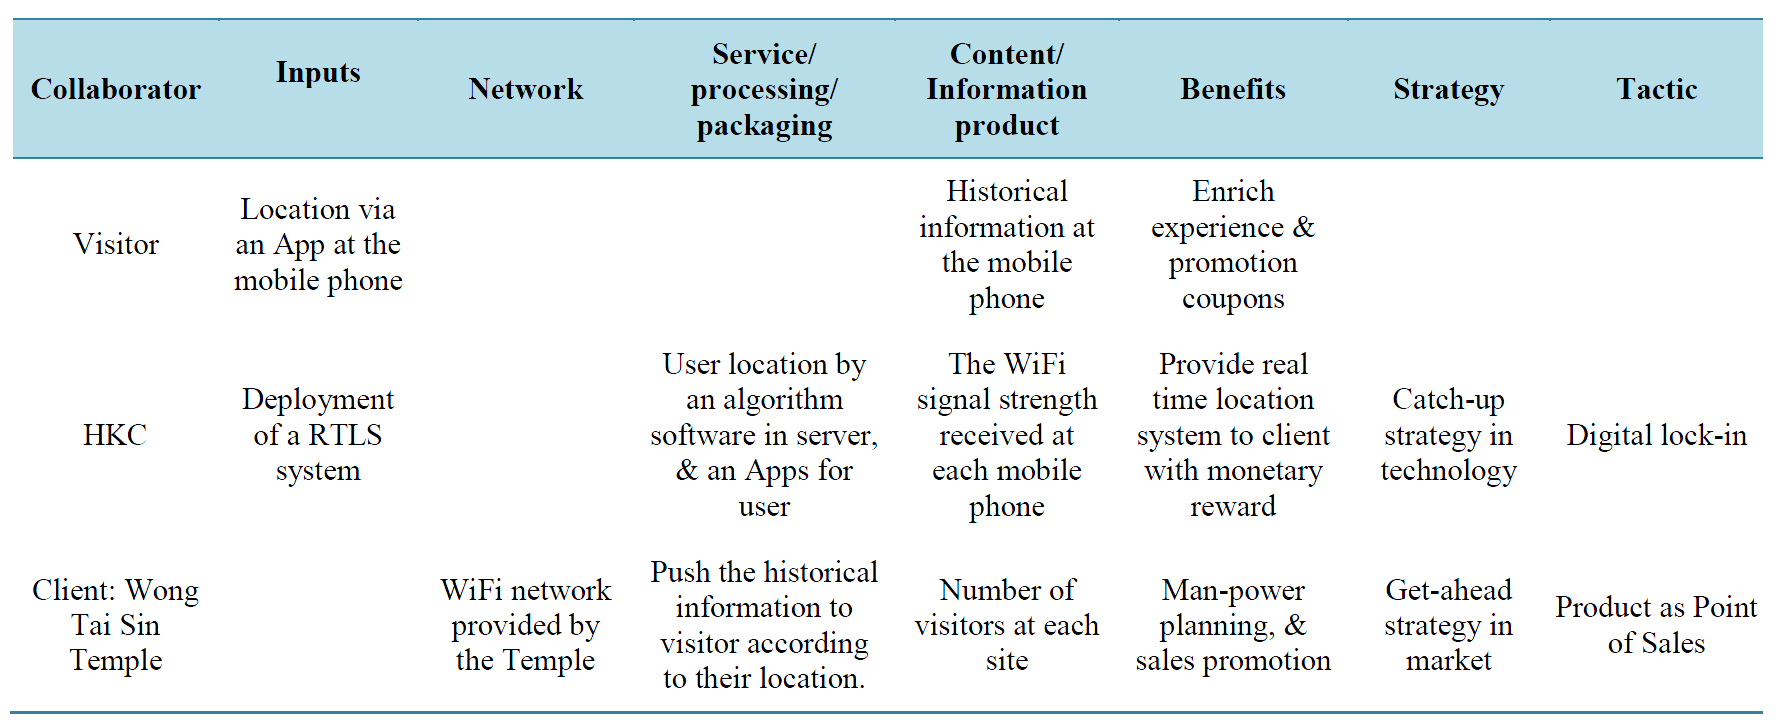
\includegraphics[scale=0.5]{Talk11/chanexample.png}
		    \end{center}
		    \caption{Chan's business model framework}
		    \label{Chan exmaple}
		\end{figure}

		Figure \ref{Chan exmaple} shows the according business model. Interesting are the fields strategy and tactic. Li et al.,(2012) \cite{li} proposed four IoT strategy categories which are adapted by Chan in the use cases for his three dimensional business model framework. The categories are: get-ahead strategy in market, catch-up strategy in market, get-ahead strategy in technology, and catch-up strategy in technology. Get-ahead strategies enable the firm to stay ahead of other competitors, giving them to first mover advantage. Catch-up strategies on the other hand follow and learn from the industrial leaders by operational efficiency and quality \cite{chan}.
		Besides strategy, the business model framework contains the component tactic. Six components of the digitally charged products by Fleisch et al.\cite{fleisch} enrich the framework:

		\begin{itemize}
			\item Physical Freemium: physical asset with free digital service, premium charged service offered.
			\item Digital Add-on: cheap physical asset, digital services can be bought or activated at a high margin.
			\item Digital lock-in: limit compatibility, high dependency, unable to use another service without high switching costs.
			\item Product as Point of Sales: physical products become  sites of digital sales and marketing services.
			\item Object Self-Service: `things' can place orders autonomously over the Internet. 
			\item Remote Usage and Condition Monitoring: smart things collect and send data in real time which enables real time monitoring and error prevention.
		\end{itemize}

		The three dimensional collaborator model by Chan is less abstract than the ecosystem framework by Westerlund et al. \cite{westerlund}. It is tested and ready to use as the use cases prove.

	% \begin{itemize}
	% 	\item Explain changes in Business Models due to IoT Development
	% 		\begin{itemize}
	% 				\item From ``Designing Business Models for the Internet of Things'' \cite{westerlund}
	% 			\begin{itemize}
	% 				\item Explains how ecosystem business models can be designed (Value Design) to show ``the dynamics between the components'' or ``ow the engine works''

	% 				\begin{enumerate}[I]
	% 					\item \textbf{Value Drivers}
	% 					\begin{itemize}
	% 						\item Individual motivations
	% 						\item Shared motivations
	% 					\end{itemize}
	% 					\item \textbf{Value Nodes}
	% 					\begin{itemize}
	% 						\item Actors
	% 						\item Activities
	% 						\item (Automated) processes
	% 					\end{itemize}
	% 					\item \textbf{Value Exchanges}
	% 					\begin{itemize}
	% 						\item Resources
	% 						\item Knowledge
	% 						\item Money
	% 						\item Information
	% 					\end{itemize}
	% 					\item \textbf{Value Extracts}
	% 					\begin{itemize}
	% 						\item Monetization
	% 					\end{itemize}					
	% 				\end{enumerate}
	% 			\end{itemize}
	% 			\item From ``IEEE-SA Internet of Things (IoT) Ecosystem Study'' \cite{cisco}
	% 				\begin{itemize}
	% 					\item IoT Ecosystem
	% 						\begin{enumerate}[I]
	% 							\item \textbf{Where does IoT stand today}
	% 								\begin{itemize}
	% 									\item Players
	% 									\item Market
	% 									\item Technology
	% 									\item Standardization
	% 								\end{itemize}
	% 							\item \textbf{Business Model View}
	% 								\begin{itemize}
	% 									\item New segments
	% 									\item Open issues / Insufficiency
	% 								\end{itemize}		
	% 						\end{enumerate}
	% 				\end{itemize}
	% 			\item From ``Business Models and the Internet of Things'' \cite{fleisch}
	% 				\begin{itemize}
	% 					\item Based on 55 different business models patterns \cite{gassmann}
	% 					\item IoT Business Model 1: Digitally Charged Products
	% 						\begin{itemize}
	% 							\item A digitally charged product ``links digital services to physical products to create a hybrid bundle that is a single whole.''
	% 							\item \textbf{Components}
	% 								\begin{enumerate}[a]
	% 									\item Business Model View
	% 									\item Physical Freemium
	% 									\item Digital Add-on
	% 									\item Digital Lock-in
	% 									\item Object Self Service
	% 									\item Remote Usage and Condition Monitoring
	% 								\end{enumerate}
	% 						\end{itemize}
	% 					\item IoT Business Model 2: Sensor as a Service
	% 						\begin{itemize}
	% 							\item A sensor as a service business model is based on ``collecting, processing and selling for a fee the sensor data [...]''.
	% 						\end{itemize}
	% 				\end{itemize}
	% 		\end{itemize}
	% \end{itemize}

\section{Comparison of available IoT Business Model Frameworks using a case study}
\label{sec:bmf_comparison}
	In the following section, we will introduce a fictitious company in order to make it possible to compare the available business model frameworks and illustrate their respective strengths and weaknesses.

	Business models for IoT differ from traditional business models. This section takes a look at what changed due to the emergence of IoT.

	In the ecosystem business model framework by Westerlund et al. \cite{westerlund} there is dogmatic shift. The business model is not seen on the level of a single company like traditional business models traditionally are. Rather, the concept of value design can be applied at the ecosystem level. Such a conception of business models in an ecosystem may be more suitable considering the nature of IoT. Networking, interconnections, interconnectivity and thus interdependence come with the territory when talking about IoT. IoT in itself is an ecosystem that can be scaled from only personal devices like wearables to huge networks like smart cities. In smart cities there are many actors and stakeholders. Identifying ecosystems within a smart city and thus finding shared and private value drivers allow businesses to cooperate efficiently with each other in a win-win environment. Traditional business model lack an ecosystem view. With ecosystem business model frameworks an important and inherent to IoT aspect can be addressed and monetized on that other traditional business models fail to reach. Naturally such a business model becomes more complex and skilled managers are needed for a successful implementation. The focus from the firm level needs to be extended to a broader view. Connections to new industries have to be made which is not an easy task, but is needed for businesses to break into the new IoT market and prove themselves and offer their customer value.

	Nevertheless, the ecosystem business model framework also shares some similarities to traditional business model frameworks. In the core, value design is a concept found in many business models. As can be seen in the magic triangle by Gassmann \cite{gassmann55}, value is one of the nodes that make up the magic triangle and is thus essential for the business model to work. Furthermore the pillars in the ecosystem business model framework can be categorized, compared and examined like the building blocks of other business models frameworks as the vertices in the magic triangle or the building blocks of the business model canvas.

	However, the ecosystem business model framework may be to abstract to be yet applied to businesses, whereas  Chan's three dimensional collaborator framework proves is usefulness in the use cases. Similar to the ecosystem business model it focuses on the multitude of actor who benefit from each other. Besides the emphasis on collaborators, concrete benefits for all are captured in the model and new components strategy and tactic enrich the model. While traditional business models may work for IoT companies, Chan's  business model framework is specifically tailored for the needs of IoT companies. Sticking to the business model canvas, Dijkman et al. \cite{dijkman} don't bring a new framework per se, but rather show relative importance of the individual building blocks. Unsurprisingly, the value proposition building block has by far the highest relative importance compared to the other block. Generally speaking an emphasis on value creation and capture as well as an emphasis on a more networked environment can be observed. Hui \cite{hui} states that in industries that are becoming connected, differentiation, cost, and focus are no longer mutually exclusive but rather can be mutually reinforcing in creating and capturing value.

	\subsection{Introduction to the case study company}
		Our case study company is called `FlexSpace' that offers a integrated beacon and software solution for companies to make the usage of companies' office space more flexible by showing the available desk places in an office to employees. This allows the customer companies to increase the usage of their office and thereby reduce the square meters per employee which directly saves money for the company. A beacon is a miniature, battery-powered sender that usually uses the Bluetooth Low Energy (BLE) technology to communicate with nearby devices. These beacons allow to let the employees check-in at their desk using their smartphones. `FlexSpace' offer the installation and maintenance of the described beacon infrastructure at customer sites as well as a white-label mobile application for their customers. The application displays the available desk places and enables the user to check-in at a specific desk using the closest beacon available. The visual appearance can be customized per customer to fit the customer company's corporate design.

	%\subsection{IoT Business Model Patterns (Fleisch et. al, 2014)}

	\subsection{Adapted Business Model Canvas for IoT (Dijkman et. al, 2015)}

	\subsection{Ecosystem Business Model Value Pillars (Westerlund et al., 2014)}
		Westerlund et al. suggest ``that managers need to shift their focus from `the business model' of a firm" to `ecosystem business models''' \cite[p. 8]{westerlund}. The application of the framework proposed by them leads us to the following business model for FlexSpace:

		Value Drivers: Sustainability (less office space per employee), increased employee satisfaction (employee can choose his own desk place) and availability of usage data

		Value Nodes: FlexSpace Employee, Beacons, Beacon Manufacturer, Beacon Installation Partner, Managers, Employees, Office Usage Application (data processing), Internal IT department

		Value Exchanges: Beacon from manufacturer to Location from employee to beacon, data from beacon to office usage application, information from office usage application to manager, knowledge from FlexSpace Employee to Manager

		Value Extract: Installation Process, Software Licensing, Provision from installation partners, Training fees to learn how to use the Office Usage Application

	\subsection{Three-dimensional collaborator Model (Chan, 2015)}

		

\section{Evaluations and Discussion}
\label{sec:eval}
	% \begin{itemize} 
	% 	\item Partly based on outcome of discussion within the seminar
	% 	\item Critical questions regarding the relevance of the results
	% 	\item How can the conducted comparison help IoT companies to design better business models?
	% \end{itemize}

	Westerlund: FlexSpace is not a typical ecosystem business idea. Typical example would be a multi-sided platform such as the Apple AppStore. Maybe that's why the application of the framework was difficult. Also, the authors themselves stated that their paper only proposes the four key value pillars that can be used as a basis for the development of a practically applicable business model framework tool in the future.

\section{Summary and Conclusions}
\label{sec:summary}
	
	This paper presents the essentials to the `Internet of Things' paradigm and the concept of business models. Based on literature research, currently important business model frameworks for IoT businesses were presented and described. The illustrated frameworks were compared based on an imaginary model company. In the evaluation it was concluded that [...] based on [...].\\
	The literature on business models for IoT is relatively scarce, thus this paper is based on few self referencing papers e.g. \cite{ju} and \cite{dijkman} and lacks a broader view. As evaluated in Section~\ref{sec:eval} [...]\\
	To conclude [.. only more generally usable framework is canvas/dijkman... a deeper analysis of each block would lead to a more specific framework, but also only usable for a subsection of businesses ...]
	% \begin{itemize} 
	% 	\item Summarize the paper content
	% 	\item Show limitations of the paper
	% 	\item Give indications for potential future work related to the topic of this paper
	% \end{itemize}

 \begin{thebibliography}{99}
	 \bibitem {gassmann} O. Gassmann, K. Frankenberger, and M. Csik: \emph{Revolutionizing the business model.} in O. Gassmann and F. Schweitzer (Eds.), Management of the Fuzzy Front End of Innovation. Springer, New York, pp. 89-97, 2014, \url{http://link.springer.com/chapter/10.1007%2F978-3-319-01056-4_7}, last visit: October 06, 2016.

	 \bibitem {gassmann55} Gassmann et al.: \emph{Gesch�tsmodelle entwickeln: 55 innovative Konzepte mit dem St. Galler Business Model Navigator.} in Hanser Verlag, 2013.

	 \bibitem {osterwalder} A. Osterwalder, Y. Pigneur, A. Smith: \emph{Business Model Generation}, self published, 2010.

	 \bibitem {bmc} Strategyzer AG: \emph{The Business Model Canvas}, \url{https://strategyzer.com/canvas/business-model-canvas}, last visit: October 06, 2016.

	 \bibitem {dijkman} R.M. Dijkman, B. Sprenkels, T.Peeters, and A. Janssen: \emph{Business Models for the Internet of Things}, International Journal of Information Management, Vol 35, pp 672-678, 2015.

	 \bibitem {fleisch} E. Fleisch, M. Winberger, F. Wortmann: \emph{Business Models and the Internet of Things}, Bosch Internet of Things \& Services Lab, pp 1-19, August 2014, \url{http://www.iot-lab.ch/?page_id=10543}, last visit: October 06, 2016.

	 \bibitem {rossi} B. Rossi: \emph{How the Internet of Things is Changing Business Models}, Information Age - Insight and analysis for IOT leaders, May 4, 2016 \url{http://www.information-age.com/it-management/strategy-and-innovation/123461371/how-internet-things-changes-business-models}, last visit: October 06, 2016.

	 \bibitem {hui} G. Hui: \emph{How the Internet of Things Changes Business Models}, Harvard Business Review, July 24, 2014, \url{https://hbr.org/2014/07/how-the-internet-of-things-changes-business-models}, last visit: October 06, 2016.

	 \bibitem {cisco} CISCO: \emph{IEEE-SA Internet of Things Ecosystem Study}, IEEE Standards Association, New York, 2015, \url{http://www.cisco.com/c/dam/en/us/solutions/collateral/industry-solutions/dlfe-670918525.pdf}, last visit: October 06, 2016.

	\bibitem {westerlund} M. Westerlund, S. Leminen and M. Rajahonka: \emph{Designing Business Models for the Internet of Things} Technology Innovation Management Review, July 2014, \url{http://timreview.ca/article/807}, last visit: October 06, 2016.

	\bibitem {ju} Jaehyeon Ju, Mi-Seon Kim and Jae-Hyeon Ahn: \emph{Prototyping Business Models for IoT Service}, Procedia Computer Science, 91, pp. 882 - 890, 2016, \url{http://www.sciencedirect.com/science/article/pii/S1877050916312911}, last visit: October 06, 2016.
 	
 	\bibitem {tilley}  A. Tilley, Google Acquires Smart Thermostat Maker Nest For \$3.2 Billion. 2014  [cited 2016 May 15]; Available from: \url{http://www.forbes.com/sites/aarontilley/2014/01/13/google-acquires-nest-for-3-2-billion/#7049b3181416}
 	
 	\bibitem {gartner}  Gartner. 4.9 Billion Connected ``Things'' Will Be in Use in 2015. 2014  [cited 2016 May 15]; Available from: \url{http://www.gartner.com/newsroom/id/2905717}

	\bibitem {chan} Chan, H.C.Y. (2015) Internet of Things Business Models. Journal of Service Science and Management,8, 552-568. \url{http://dx.doi.org/10.4236/jssm.2015.84056}, last visit: October 06, 2016.

	\bibitem {itu} \todo{TODO}

	\bibitem {Atzori} \todo{TODO}

	\bibitem {osterwalder2005} \todo{TODO}

	\bibitem {holler} Holler, J., Tsiatsis, V., Mulligan, C., Avesand, S., Karnouskos, S. and Boyle, D. (2014) From Machine-to-Machine to the Internet of Things: Introduction to a New Age of Intelligence. Elsevier, Waltham.

	\bibitem {li} Li, Y., Hou, M.J., Liu, H. and Liu, Y. (2012) Towards a Theoretical Framework of Strategic Decision, Supporting Capability and Information Sharing under the Context of Internet of Things. Information Technology and Management, 13, 205-216.
	\url{http://dx.doi.org/10.1007/s10799-012-0121-1}, last visit: October 06, 2016.

	\bibitem {osterwalder2010} \todo{TODO}

 \end{thebibliography}

